%!TEX root =  concept_mining.tex


\begin{table*}
\small
\centering
\begin{tabular}{llllll} 
\toprule
Datasets & Task & Domain & Metric & $\vert$ Train$\vert$ & $\vert$Test$\vert$  \\
\midrule

Sample Text & \multirow{5}{*}{\begin{tabular}[c]{@{}l@{}}Text Modeling\end{tabular}}  & General text           & \multirow{5}{*}{\begin{tabular}[c]{@{}l@{}}Word prediction + \\ Next sentence prediction\end{tabular}} & 16   & 480     \\
Sample Large &                         & General text &       & 280K  & 8.4M     \\
Wikitext-2 converted       &                         & Articles from Wikipedia &   & 60K  & 1800K     \\
Arxiv Computer Science      &                         & Technical papers from \url{arxiv.org}  &       & 362K  & 1.1M     \\
Arxiv Math       &                         & Technical papers from \url{arxiv.org} &      & 175K  & 525K     \\
\midrule
CoLA & classification  & Books and journal articles  & Matthews coefficient      & 8.5k & 1k    \\
\midrule
MRPC &  \multirow{2}{*}{\begin{tabular}[c]{@{}l@{}}paraphrase\end{tabular}}  & News &  \multirow{2}{*}{\begin{tabular}[c]{@{}l@{}}Accuracy / F1\end{tabular}} 
& 3.7k & 1.7k   \\
QQP &                         & Questions from Quora &      & 364k & 391k  \\ 
\midrule
STS-B & Sentence Similarity                    & Misc.    & Pearson/Spearman       & 7k & 1.4k  \\
\midrule
MNLI        &  \multirow{2}{*}{\begin{tabular}[c]{@{}l@{}}NLI\end{tabular}}                   & Internet Crawl  & \multirow{2}{*}{\begin{tabular}[c]{@{}l@{}}Accuracy\end{tabular}}      &393k & 20k   \\
RTE      &          & Wikipedia             &      &  2.5k & 3k  \\
\midrule
QNLI     & QA + NLI & News and Wikipedia   & \multirow{2}{*}{\begin{tabular}[c]{@{}l@{}}Accuracy\end{tabular}}      & 105k & 5.4k  \\
WNLI        & coreference + NLI & Fiction books   &        & 634 & 146  \\
\bottomrule
\end{tabular}
\caption{An overview of different datasets under different classification tasks including description and sizes.}
\label{tab:dataset}
\end{table*}





\begin{figure*}
\begin{minipage}[b]{.33\linewidth}
 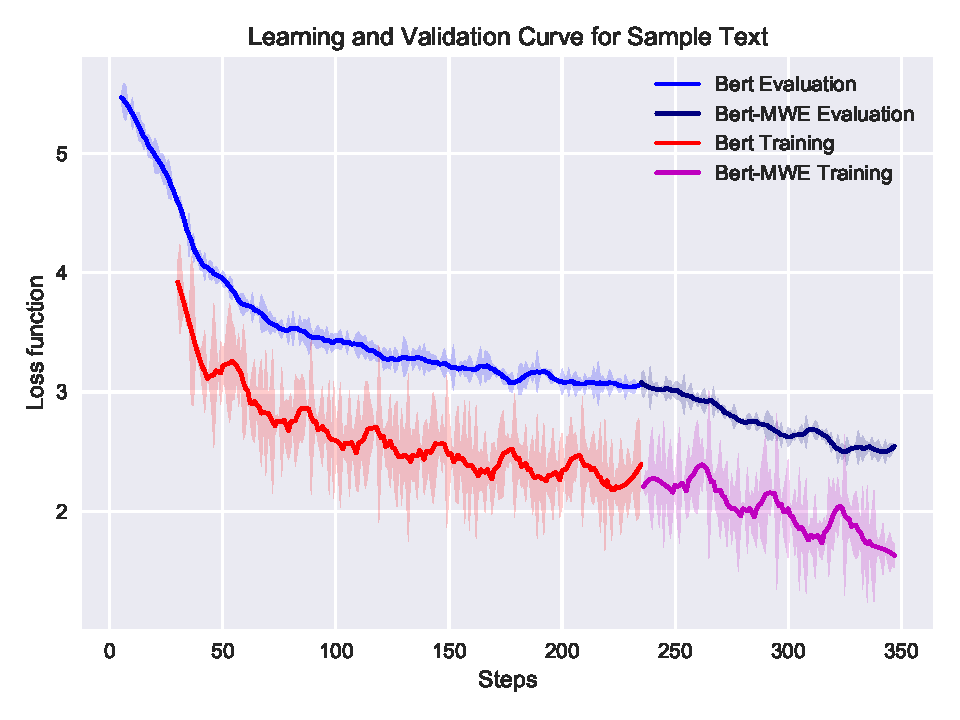
\includegraphics[width=\linewidth]{fig/st.pdf}
\label{fig:manual-eval1}
\end{minipage}
\begin{minipage}[b]{.33\linewidth}
 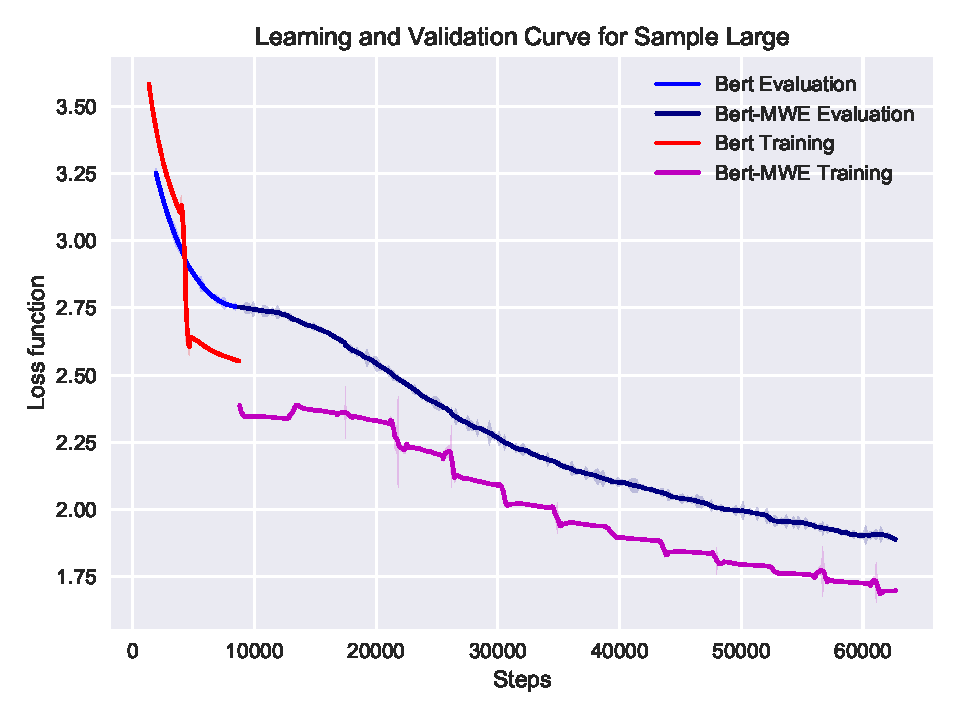
\includegraphics[width=\linewidth]{fig/sl.pdf}
\label{fig:manual-eval2}
\end{minipage}
\begin{minipage}[b]{.33\linewidth}
 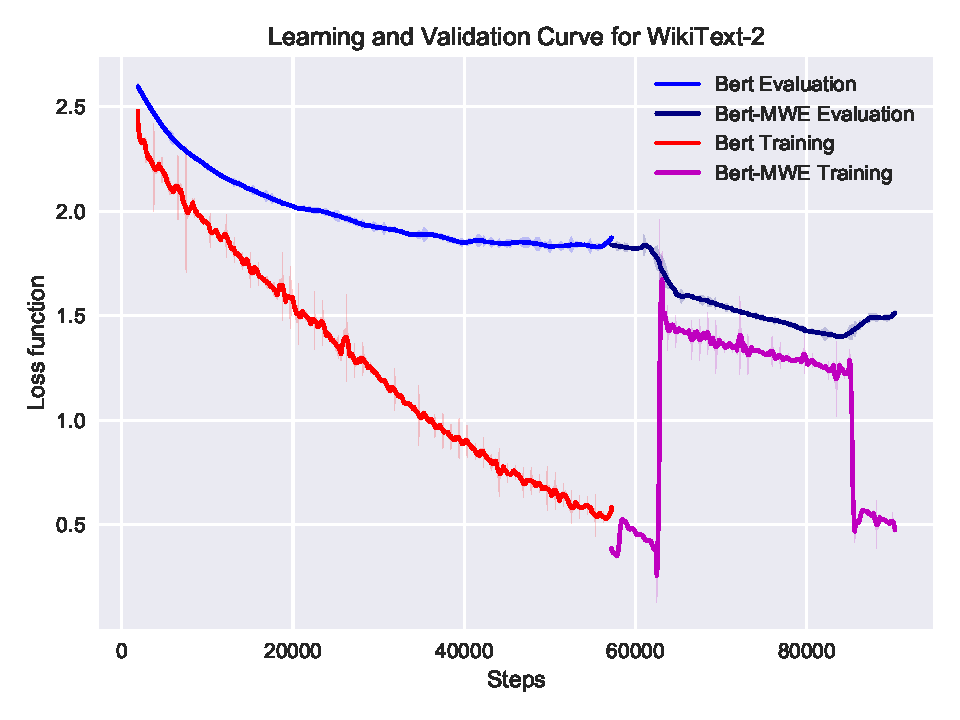
\includegraphics[width=\linewidth]{fig/w.pdf}
\label{fig:manual-eval2}
\end{minipage}
\vspace{-15pt}
\caption{Learning and validation curve for the our datasets.}
\label{fig:learning-curve}
%\vspace{3pt}
\end{figure*}





\begin{table*}
\begin{center}
\begin{tabular}{lllclcllc} 
\toprule
System      & CoLA                                                                         & MRPC                                                                              & QQP                           & STS-B              & QNLI                     & MNLI          & RTE           & WNLI                      \\ 
\hline
BiLSTM      & 11.6                                                                         & 81.8/74.3                                                                         & \multicolumn{1}{l}{62.5/84.2} & 70.3/67.8          & \multicolumn{1}{l}{74.6} & 65.6          & 57.4          & \multicolumn{1}{l}{65.1}  \\
BiLSTM+Attn & \textcolor[rgb]{0.133,0.133,0.133}{\textcolor[rgb]{0.133,0.133,0.133}{18.6}} & \textcolor[rgb]{0.133,0.133,0.133}{\textcolor[rgb]{0.133,0.133,0.133}{83.9/76.2}} & 72.8/70.5                     & 72.8/709           & 74.3                     & 67.6          & 58.4~ ~~      & 65.1                      \\
OpenAI GPT  & 45.4                                                                         & 82.3/-                                                                            & 70.3/-                        & 80.0/-             & 87.4                     & 82.1          & 56.0          & 65.1                      \\
Bert        & 57.9                                                                         & 86.0/89.9                                                                         & 89.9/86.7                     & 89.6/89.2          & 90.8                     & 83.4          & 67.1          & 57.7                      \\
\BertMWE-Simple     & 58.1                                                                         & 86.0/89.9                                                                         & 90.7/87.5                     & \textbf{90.0}/89.5 & 91.3                     & \textbf{84.0} & \textbf{72.2} & 56.3                      \\
    \BertMWE        & \textbf{59.7}                                                                & \textbf{86.5/90.4~}                                                               & \textbf{90.9/87.7}            & \textbf{90.0/89.6} & \textbf{91.5}            & \textbf{84.0} & \textbf{72.2} & \textbf{63.4}             \\
\bottomrule
\end{tabular}

   \caption{Performance on supervised label prediction}
   \label{tab:glue_results}
\end{center}
\end{table*}



\section{Experiments}\label{sec:experiments}

In this section we experimentally evaluate the proposed approach over an wide range of tasks across different domains and demonstrate its effectiveness over the state of the art baseline approaches.




\subsection{Setup}

\noindent \textbf{Hardware Environment}
The model training and preprocessing is conducted on a lab server with 3 
GeForce RTX 2080 GPU card, 2 6-core Intel(R) Core(TM) i7-6800K CPU @ 3.40GHz CPU with 12GB memory. The longest experiments took no more than 3 days.


\noindent \textbf{Model architecture and hyper-parameter settings}
Since the proposed \BertMWE approach is built upon the Bert self-attention network architecture \cite{devlin2018bert},
and 
we're mainly interested in how much it can \textit{improve} upon the basic Bert model, 
we follow the exact same architecture, hyper-parameter and optimizer settings as suggested by 
\cite{devlin2018bert} for each specific tasks 
refer the reader to the original paper for details about the architecture and parameter.

\noindent \textbf{Model training and weight initialization}
In order to more directly see the difference between the \BertMWE and the basic case Bert model, we will conduct the model training of \BertMWE in an \textit{incremental} fashion:
we first follow the best training settings for each different variant of the Bert model  to train the basic model for a specific downstream task; after that, we start to train the corresponding \BertMWE 
for the Bert variant, and use the trained weighted of base Bert model for that task to initialize the \BertMWE model. In other words, the pre-trained weights of \BertMWE come from the corresponding Bert model without MWE.

\noindent \textbf{Model variants}
we apply the \BertMWE approach over the two different variants of the original Bert as proposed in \cite{devlin2018bert}: the Bert-Finetune as described in Section 3.5 of \cite{devlin2018bert}, where we use the pretrained weights as initialization, and fine-tune the model end to end, and the Bert-Feature, where we freeze the pretrained the model weights and use the outputted hidden states as feature to train a specific classification head. We also 
explore two different version of applying the non-compositionality information.
The first is the theoretically sounded \BertMWE, which fully follows the variational inference procedure and learns a distribution of possible Bert models, as shown in \autoref{sec:var-param}; the second is a simplified version of \BertMWE, 
which do not explicitly utilize the inference, and only concat the MWE with the original single word based input. However, it may implicitly conduct inference over the importance of multiword expressions by dynamically scale their inputted embedding to the downstream network.

\subsection{Text modeling} \label{sec:dataset}
We first evaluate the proposed approach on how well it can model the text data itself, without using any supervision signal.
Specifically, we construct the training and evaluation set by following the construction of masked language model and next sentence prediction task in the orignal Bert model \cite{devlin2018bert}, and additionally, to make the competition fair with basic Bert models, 
we will discard from the input any MWEs that has overlap with the masked position. 
Any training instances whose token masked is included in the evaluation dataset is discarded.

Both the training objective function and the evaluation metric of this task will be the sum of the  masked language model objective and next sentence prediction objective, which is computed as the sum of the mean masked LM likelihood and mean next sentence prediction likelihood

We have evaluated our approach over the following corpus covering several different domains, as listed below.
The dataset statistics are shown in \autoref{tab:dataset}. 


\begin{table*}[thbH]
\centering
\small
\begin{tabular}{lcccccc} 
\toprule
Datasets                                  & Training strategy                & Methods   & Evaluation~Loss ~ & Improvement            & ~Training Loss~        & Improvement              \\ 
\midrule
\multirow{6}{*}{Sample Text} & \multirow{2}{*}{Bert Finetune} & Base   & 0.39                & -                      & 0.001                     & -                        \\
                                               &                                & \BertMWE         & 0.290                & -25.7\%           & 0.000            & -66.7\%              \\
\cline{2-7}
                                               & \multirow{2}{*}{Bert Feature}  & Base  & 3.272                & -                      & 2.074                     & -                        \\
&                                & \BertMWE      & 2.35                & -28.2\%                      & 1.139                     & -45.1\%                       \\ 
\midrule
\midrule
\multirow{6}{*}{Sample Large} & \multirow{2}{*}{Bert Finetune} & Base   & 2.768                & -                      & 2.552                     & -                        \\
                                               &                                & \BertMWE      & 1.866                & -32.1\%                      & 1.670                     & - 34.56\%                       \\ 
\cline{2-7}
                                               & \multirow{1}{*}{Bert Feature}  & Base & 3.991                & -                      &         3.712            & -                        \\
                                               &                                & \BertMWE         & 3.918                 & -1.8\%           & 3.654            & -1.6\%              \\
\midrule
\midrule
\multirow{6}{*}{WikiText-2} & \multirow{2}{*}{Bert Finetune} & Base   & 1.851                & -                      & 0.588                                & -                        \\
&                                & \BertMWE      & 1.390                & -24.9\%                      & 0.489          & -16.8\%                       \\ 
\cline{2-7}
                                               & \multirow{2}{*}{Bert Feature}  & Base & 2.700                & -                      & 2.511                     & -                        \\
                                               &                                & \BertMWE         & 2.669                & -1.1\%           & 2.491            & -0.8\%              \\
\midrule
\midrule
\multirow{6}{*}{Arxiv CS} & \multirow{2}{*}{Bert Finetune} & Base   & 2.560                & -                      & 2.336                     & -                        \\
                                               &                                & \BertMWE      & 2.137                & -16.5\%                      & 1.859                     & -20.4\%                       \\ 
\cline{2-7}
                                               & \multirow{2}{*}{Bert Feature}  & Base & 3.306                & -                      & 3.072                     & -                        \\
                                               &                                & \BertMWE         & 3.277                & -0.9\%           &  3.049            & -0.7\%              \\
\midrule
\midrule
\multirow{6}{*}{Arxiv Math} & \multirow{2}{*}{Bert Finetune} & Base   & 1.658                & -                      & 1.399                     & -                        \\
                                               &                                & \BertMWE      & 1.649                & -0.5\%                      & 1.399                     & -0\%                       \\ 
\cline{2-7}
                                               & \multirow{2}{*}{Bert Feature}  & Base & 3.131                & -                      & 2.928                     & -                        \\
                                               &                                & \BertMWE         & 3.024                & -3.4\%           & 2.813            & -3.9\%              \\
\midrule
\bottomrule
\end{tabular}
\caption{Experimental Results on text modeling}
\label{tab:text_modeling}
\end{table*}





%We follow the original pre-training procedure for finetuning and evaluating different approaches, by first pre-processing the input corpus following the mask-sample-replace procedure for training the masked language model, and using the the sum of the mean masked LM likelihood and mean next sentence prediction likelihood as the objective function. 
%In order to have a fair comparison for the MWE based approaches, we prevent the information "leakage" from the MWE in the sentence that may contain the masked tokens, by discarding in the masking stage any MWE in the input if there is any overlap between the MWE and the masked tokens. The evaluation metric is then obtained by measuring the same objective function as in the training set as in a separate evaluation set.
%We carry out the text modeling task capability over several representative dataset across various domains, as described by the datasets listed below. 


%We have collected the following corpus, covering the domain of computer science, physics \& mathematics and medicine.
% The statistics of these datasets are summarized in Table S1, and the details are described below.

\noindent \textbf{Sample Text} 
We first test the validity of our approaches over a simple 30-sentence corpus
obtained from the commonly adopted Pytorch implementation of Bert repository \footnote{\url{https://github.com/huggingface/pytorch-pretrained-BERT/blob/master/samples/sample_text.txt}}.


\noindent \textbf{Sample Large}
The Sample Large corpus is also provided by Pytorch Bert repository  \footnote{\url{https://github.com/huggingface/pytorch-pretrained-BERT/blob/master/samples/sample_text.txt}}
which consists of about 500K natural language text to test the validity of our approaches in a large scale setting.
\footnote{\url{https://ext-bert-sample.obs.eu-de.otc.t-systems.com/small_wiki_sentence_corpus.txt}}

\noindent \textbf{WikiText-2} 
The WikiText-2 corpus is a cleaned Wikipedia corpus proposed by Merity et.al \cite{merity2016pointer} as a standard benchmark for language model in the general domain. 
Although larger version of the Wikipedia corpus exists, we adopt the WikiText-2 as the benchmark because the model is already initialized with the weights pretrained from the entire Wikipedia \cite{devlin2018bert} and therefore introduciing larget training corpus will not provide much more information.


\noindent \textbf{Arxiv Computer Science} We evaluate the performance of our approaches for modeling text for technical domains, which obtained by crawling titles and abstracts of 70K the papers from the open access repository \url{arxiv.org} under the top level category of computer science from 2008 to 2018. 


\noindent \textbf{Arxiv Maths} We also collect another dataset from the repository \url{arxiv.org}, which is obtained by crawling about 65K paper abstracts from \url{arXiv.org}, under the top level category "mathematics". 


\subsection{Supervised label prediction}
we next evaluate the proposed approaches over an array of tasks that will take the text as input and learn to predict additional supervision labels to solve downstream analytical tasks. 
For this we follow the standard the benchmark setting of 
General Language Understanding Evaluation \cite{wang2018glue}, which is a collection of many supervised label prediction tasks for natural language text.
Since GLUE does not distribute labels for the Test set and original evaluation was measured on the dev set \cite{devlin2018bert}, we use the evaluation metrics on the dev set as the Test performance. 
Specifically, we choose to evaluate our methods over the following dataset.

\noindent \textbf{CoLA} The Corpus of Linguistic Acceptability is a binary classification task for binary text classification,
where given a single sentence, the goal is to predict whether it is grammatically acceptable. We follow the author \cite{wang2018glue} to use Mathews correlation coefficient as the evaluation metric.

\noindent \textbf{MRPC} The Microsoft Research Paraphrase Corpus is a collection of sentence pairs from online news sources for paraphrase detection. Given a pair of sentence, the goal is to predict whether they are semantically equivalent. 
Because the classes are imbalanced, the author \cite{wang2018glue} suggest to use both accuracy and F1 score.


\noindent \textbf{QQP} The Quora Question Pairs dataset is another text similarity  dataset consisting of pair of questions from Quora, which follows the same from as \textbf{MPRC}. It also has imbalanced classes and therefore both accuracy and F1 score are reported.


\noindent \textbf{STS-B} 
The Semantic Textual Similarity Benchmark is a yet another paraphrase detection dataset from news headlines,  video and image captions and natural language inference data. Given a pair of sentence, the goal is to predict a score from 1 to 5 measuring the strength of their semantic similarity. The author \cite{wang2018glue} suggest to use Pearson and Spearman correlation coefficients as the performance measure.


\noindent \textbf{MNLI} The Multi-Genre Natural Language Inference dataset is a crowdsourced collections of entailment classification data collected by William et.al. \cite{williams2017broad}. 
Given a pair of sentences, the goal is to predict whether the first sentence (premise) entails or contradicts the second sentence(hypothesis), or neither of the above.

\noindent \textbf{QNLI} The Question Natural Language Inference dataset is a converted version of the Stanford Question Answering Dataset where given a pair of question and sentence, the goal is to predict whether the sentence contains the answer to the question.

\noindent \textbf{RTE} The Recognizing Textual Entailment dataset is a collection of entailment dataset in the same form as \textbf{MNLI} constructed based on news and Wikipedia.

\noindent \textbf{WNLI} The Winograd Natural Language Inference dataset is converted from Winograd Schema Challenge whetre goal is to determine the the referent of pronouns in the given sentence. Given a input pair of sentence, the goal is predict whether the second sentence is equivalent to the first one, by replacing the pronoun with the correct referent.




\subsection{Performance evaluation}
\noindent \textbf{Text modeling}
We first evaluate our approach over the task of modeling the text, under the Bert-pretraining objective \cite{devlin2018bert}, the results are shown in \autoref{tab:text_modeling}. We omit the the \BertMWE-simple model for clearity because it generate similar performance with the \BertMWE, possibly because it can scale its embedding parameters to simulate the dropout behavior.
We can see from the results that \BertMWE model is able to efficiently utilize the training set, (by reducing the training error), while at the same time significantly reduce the loss on evaluate set on most of the benchmarks. Another observation is that, the \BertMWE, when it achieves similar performance over the evaluation, it also behaves similarly on the training set. In other words, adding the additional will mostly not lead to overfitting, and in many cases, let the model learn better structure of the data.

\noindent \textbf{Supervised label prediction}
We evaluate our approach over the task of predicting the external supervised labels, as shown in table \autoref{tab:glue_results},
where we list the performance of each several Bert based models along with several additional methods results obtained from the Glue online benchmark to serve as reference.
We can see the \BertMWE is able to build upon the already very strong Bert base model, and achieve statistically significant improvement over a wide range of tasks, and outperform other strong baseline methods.





\subsection{Case study}






To provide further insights about the learning process, we present the learning curve and evaluation curve for the text modeling datasets used in the performance evaluation, as shown in \autoref{fig:learning-curve}, from which we can clearly see that adding the additional structure \BertMWE gives significant impact over the base Bert model, through better exploitation of the training data as well as a significantly better generalization error.




\nop{
\noindent \textbf{Interpretation of MWE weights}
By inspecting the model weights, we can derive better,
intuitively, MWEs associated with high weights and less dropout 
valid
critical to the task
The results are shown in \autoref{table-top-concepts} shows some of the most discriminative \& indiscriminative MWEs. We can see that the concept representation of taxonomy nodes is able to capture latent semantics and make meaningful distinctions on the concept level.





\begin{table}
\centering

\resizebox{\columnwidth}{!}{%
\begin{tabular}{c|c|c} \hline
\multirow{2}{*}{} & \multicolumn{2}{c}{Concepts} \\ \cline{2-3} & discriminative & indiscriminative \\ \hline
\multirow{3}{*}{\it{\textbf{Computer Science}}} & \it{fpga (Hardware)} & \it{framework} \\ & \it{nash 
equilibria (Game Theory)} & \it{goal} \\ & \it{attacks (Security)} & \it{technique} \\ \hline
\multirow{3}{*}{\it{\textbf{Physics & Maths}}} & \it{entanglement (Quantum Physics)} & \it{correspondance} \\ & \it{Jupyter (Planet astrophysics)} & \it{metric} \\ & \it{complete graph  (Combinatorics)} & \it{series} \\
\hline
\multirow{3}{*}{\it{\textbf{Medicine}}} & \it{MRI (Diagnosis)} & \it{levels} \\ & \it{treatment (Therapeutics)} & \it{ability} \\ &  \it{HIV (Viruses)} & \it{regression} \\ \hline
\end{tabular}
}
\vspace{3pt}
\caption{Example discriminative vs indiscriminative concepts discovered in each dataset}
\vspace{-10pt}
\label{table-top-concepts}
\end{table}

}





